\section{Используемые компоненты и технологии}
\label{section:Technologies}

% **************************************************
\subsection{PDM микрофон \micname{}}
На данный момент существует огромное число различных видов микрофонов с широким спектром характеристик. Но большинство из них мало подходят для применения в микрофонных решётках. Дело в том, что обычные микрофоны выдают на выходе аналоговый сигнал и для его последующей цифровой обработки потребуется АЦП. С ростом числа микрофонов в решётке возрастёт и число микросхем АЦП, что приведёт к удорожанию и усложнению конечного устройства.

Однако, в последнее время, на рынке появились, так называемые, цифровые микрофоны. Они имеют интегрированный АЦП и выдают на выходе сигнал в PDM формате. Примером такого устройства является микрофон \micname{} от фирмы ST. Его внешний вид представлен на рисунке~\ref{fig:PdmMicPhoto}

\begin{figure}[ht]
	\centering
	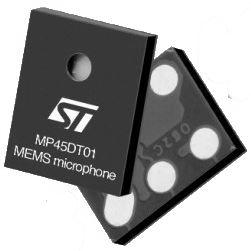
\includegraphics[scale=1.2]{PdmMicPhoto.jpg}  
	\caption{Микрофон \micname{}}
	\label{fig:PdmMicPhoto}
\end{figure}

\subsubsection{Возможности. }
Фирма ST заявляет следующие возможности микрофона \micname~\cite{ST_MP45DT02}:
\begin{itemize}
	\item Для работы необходимо только одно напряжения питания;
	\item Низкая потребляемая мощность при работе;
	\item Всенаправленная чувствительность;
	\item Однобитный выход с возможностью работы в стерео-режиме;
	\item Металлический или пластиковый HLGA корпус для поверхностного монтажа.
\end{itemize}

\subsubsection{Характеристики. }
Микрофон \micname{} обладает следующими характеристиками~\cite{ST_MP45DT02}:
\begin{itemize}
	\item Напряжение питания 1,64--3,6 В;
	\item Потребляемый ток в рабочем режиме 0,65 мА;
	\item Отношение сигнал-шум 61 дБ;
	\item Чувствительность -26 дБ;
	\item Максимальная тактовая частота 3,25 МГц.
\end{itemize}

Амплитудно-частотная характеристика данного микрофона изображена на рисунке~\ref{fig:PdmMicResponse}

\begin{figure}[ht]
	\centering
	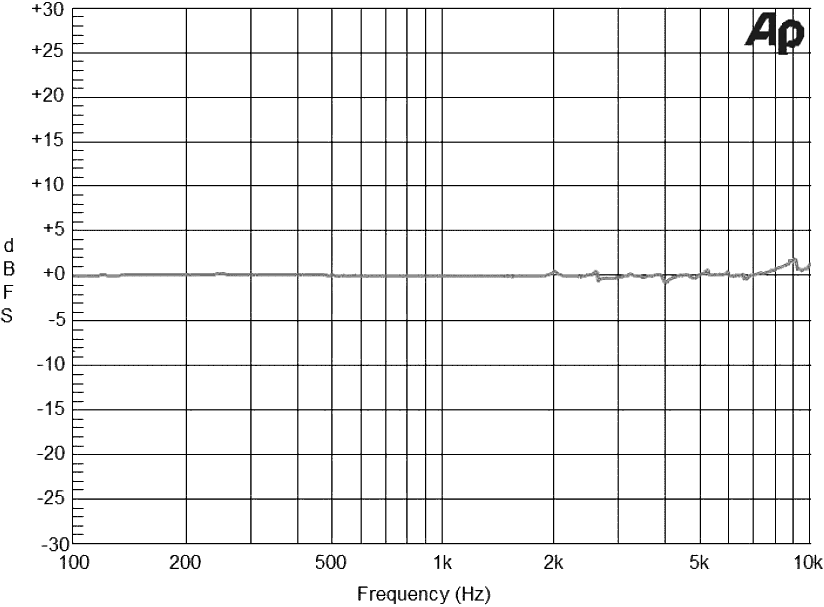
\includegraphics[scale=0.75]{PdmMicResponse.png}  
	\caption{Амплитудно-частотная характеристика микрофона \micname{}}
	\label{fig:PdmMicResponse}
\end{figure}

\subsubsection{Применение. }
Микрофон \micname{} может применяться в таких областях как~\cite{ST_MP45DT02}:
\begin{itemize}
	\item Мобильные терминалы;
	\item Ноутбуки и портативные компьютеры;
	\item IP-телефония;
	\item Распознавание речи;
	\item Игровые устройства и устройства виртуальной реальности;
	\item Цифровые видеокамеры;
	\item Охранные системы.
\end{itemize}

\subsubsection{Краткое описание. }
\micname{}~--- это компактный, потребляющий небольшое количество энергии, всенаправленный микрофон с верхним расположением звукового отверстия. В данный микрофон встроен чувствительный элемент и цифровой интерфейс с возможностью работы в стерео-режиме~\cite{ST_MP45DT02}.

Чувствительный элемент, способный регистрировать акустические волны, произведён с использованием специального процесса микрообработки кремния~\cite{ST_MP45DT02}.

Встроенная интегральная микросхема, произведённая по CMOS технологии, позволяет получать с микрофона сигнал в PDM формате~\cite{ST_MP45DT02}.

\micname{} имеет акустическую точку перегрузки в 120 дБ с лучшим на рынке отношением сигнал/шум 61 дБ и чувствительностью $-20$~дБ
Встроенная интегральная микросхема, произведённая по CMOS технологии, позволяет получать с микрофона сигнал в PDM формате~\cite{ST_MP45DT02}.

\micname{} доступен в SMD-совместимом металлическом либо пластиковом корпусе с гарантией функционирования в расширенном диапазоне температур от $-30\,^{\circ}{\rm C}$ до $85\,^{\circ}{\rm C}$~\cite{ST_MP45DT02}.

Цифровой выход и небольшие размеры корпуса (толщина всего 1,25~мм) делают данный микрофон наилучшим решением для переносных вычислительных устройств~\cite{ST_MP45DT02}.

\subsubsection{Схема подключения. }
Каждый микрофон \micname{} оснащён последовательным интерфейсом для считывания данных в формате PDM.
 
Данный последовательный интерфейс состоит из входа для тактирования цифровой части микрофона и выходом данных. Для возможности подключения двух микрофонов на одну шину данных в микрофоне \micname{} предусмотрен конфигурационный вход, позволяющий задавать момент, когда на выходе данных микрофона появится информация. Согласно документации на микрофон~\cite{ST_MP45DT02}, при подаче на конфигурационный вход логической единицы, данные будут появляться на выходе по переднему фронту тактового сигнала. При подаче на конфигурационный вход логического нуля, данные появятся по заднему фронту тактового сигнала (рисунок~\ref{fig:PdmMicWaveform})
 
\begin{figure}[ht]
	\centering
	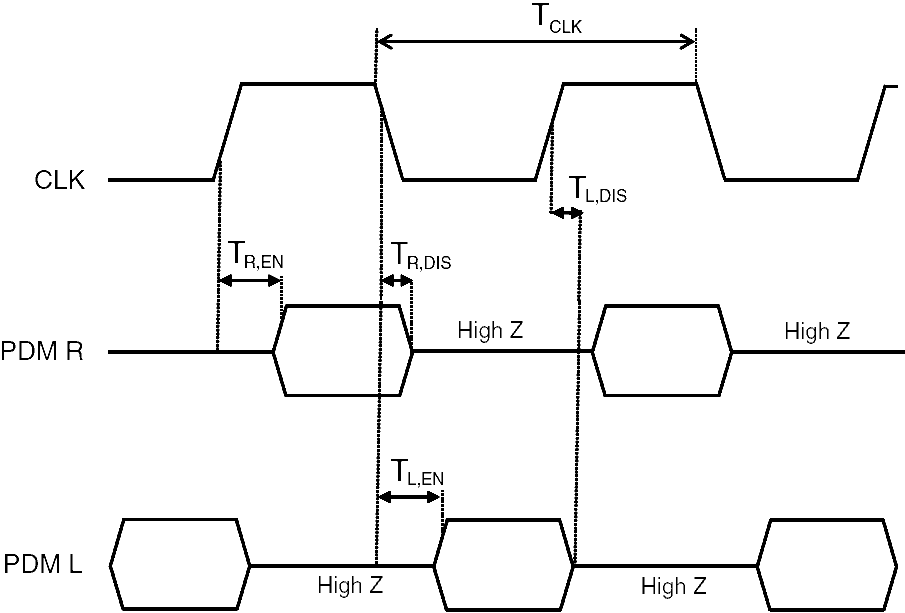
\includegraphics[scale=0.6]{PdmMicWaveform.png}  
	\caption{Форма тактового и выходного сигнала микрофона \micname{}}
	\label{fig:PdmMicWaveform}
\end{figure}
 
Типичная схема подключения двух микрофонов на одну шину данных показана на рисунке~\ref{fig:DoublePdmMic}

\begin{figure}[ht]
	\centering
	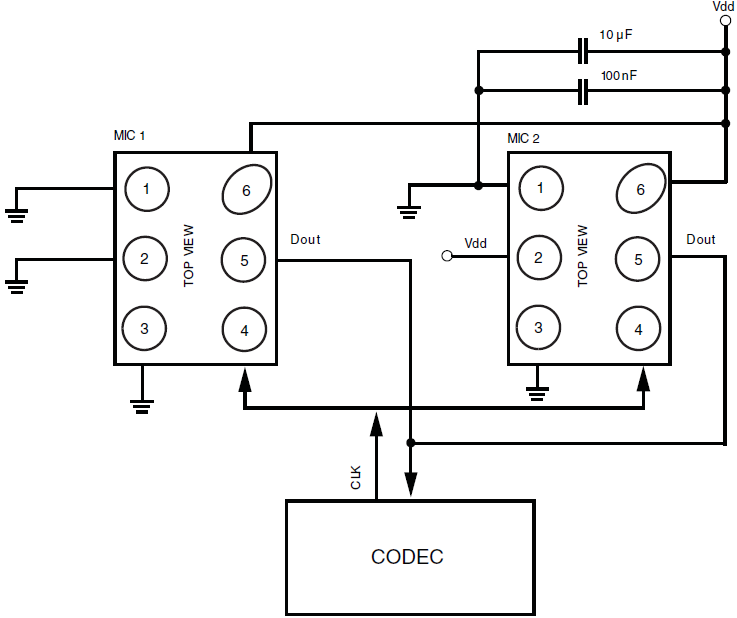
\includegraphics[scale=0.7]{DoublePdmMic.png}  
	\caption{Схема подключения двух микрофонов на одну шину данных}
	\label{fig:DoublePdmMic}
\end{figure}


% **************************************************
\subsection{Программируемые пользователем вентильные матрицы}

Программируемая логическая интегральная схема (ПЛИС, англ. \foreignlanguage{english}{programmable logic device, PLD})~--- электронный компонент, используемый для создания цифровых интегральных схем. В отличие от обычных цифровых микросхем, логика работы ПЛИС не определяется при изготовлении, а задаётся посредством программирования (проектирования). Для программирования используются программаторы и отладочные среды, позволяющие задать желаемую структуру цифрового устройства в виде принципиальной электрической схемы или программы на специальных языках описания аппаратуры, таких как~\cite{Wiki_PLD}:
\begin{itemize}
	\item Verilog;
	\item SystemVerilog;
	\item VHDL;
	\item AHDL.
\end{itemize}
	
Альтернативой ПЛИС являются следующие технологии~\cite{Wiki_PLD}:
\begin{itemize}
	\item Программируемые логические контроллеры (ПЛК);
	\item Базовые матричные кристаллы (БМК), требующие заводского производственного процесса для программирования;
	\item ASIC~--- специализированные заказные большие интегральные схемы (БИС), которые при мелкосерийном и единичном производстве существенно дороже;
	\item Специализированные компьютеры, процессоры (например, цифровой сигнальный процессор) или микроконтроллеры, которые из-за программного способа реализации алгоритмов в работе медленнее ПЛИС.
\end{itemize}

Существует множество различных типов ПЛИС:
\begin{itemize}
	\item PAL;
	\item GAL;
	\item CPLD;
	\item FPGA.
\end{itemize}

Из вышеперечисленных типов ПЛИС наиболее широкими возможностями обладают FPGA.

\subsubsection{FPGA. }
\label{section:FPGA}
Программируемая пользователем вентильная матрица (ППВМ, англ. \foreignlanguage{english}{Field-Programmable Gate Array, FPGA})~--- полупроводниковое устройство, которое может быть сконфигурировано производителем или разработчиком после изготовления; отсюда название: <<программируемая пользователем>>. ППВМ программируются путём изменения логики работы принципиальной схемы, например, с помощью исходного кода на языке проектирования (типа VHDL), на котором можно описать эту логику работы микросхемы. ППВМ является одной из архитектурных разновидностей программируемых логических интегральных схем (ПЛИС)~\cite{Wiki_FPGA}.

ППВМ могут быть модифицированы практически в любой момент в процессе их использования. Они состоят из конфигурируемых логических блоков, подобных переключателям с множеством входов и одним выходом (логические вентили или \foreignlanguage{english}{gates}). В цифровых схемах такие переключатели реализуют базовые двоичные операции AND, NAND, OR, NOR и XOR. В большинстве современных микропроцессоров функции логических блоков фиксированы и не могут модифицироваться. Принципиальное отличие ППВМ состоит в том, что и функции блоков, и конфигурация соединений между ними могут меняться с помощью специальных сигналов, посылаемых схеме. В некоторых специализированных интегральных схемах (ASIC) используются логические матрицы, аналогичные ППВМ по структуре, однако они конфигурируются один раз в процессе производства, в то время как ППВМ могут постоянно перепрограммироваться и менять топологию соединений в процессе использования. Однако, такая гибкость требует существенного увеличения количества транзисторов микросхемы.
Логический блок классической ППВМ состоит из таблицы истинности (англ. \foreignlanguage{english}{lookup table, LUT}) на 4 входа и триггера~\cite{Wiki_FPGA} (см. рисунок~\ref{fig:FpgaCellExample}).

\begin{figure}[ht]
	\centering
	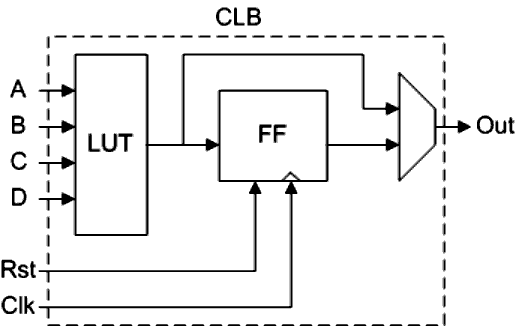
\includegraphics[scale=1.0]{FpgaCellExample.png}  
	\caption{Упрощённая схема логического блока FPGA}
	\label{fig:FpgaCellExample}
\end{figure}
 
В последние годы производители начали переходить на таблицы истинности с большим числом входов, что позволяет задействовать меньшее число логических блоков для типичных приложений.

Логический блок имеет таблицу истинности на 4 входа и вход синхронизации (\foreignlanguage{english}{clock}). Выход блока только один, это может быть регистровая или нерегистровая выходная таблица истинности. Поскольку сигналы синхронизации в коммерческих ППВМ (а часто и другие сигналы, распараллеливающиеся на большое количество входов — \foreignlanguage{english}{high-fanout signals}) трассируются особым образом специальными трассировочными цепями, управление этими сигналами делается отдельно.

Для приведённого примера архитектуры расположение контактов логического блока показано на рисунке~\ref{fig:FpgaLogicBlockPins}~\cite{Wiki_FPGA}

\begin{figure}[ht]
	\centering
	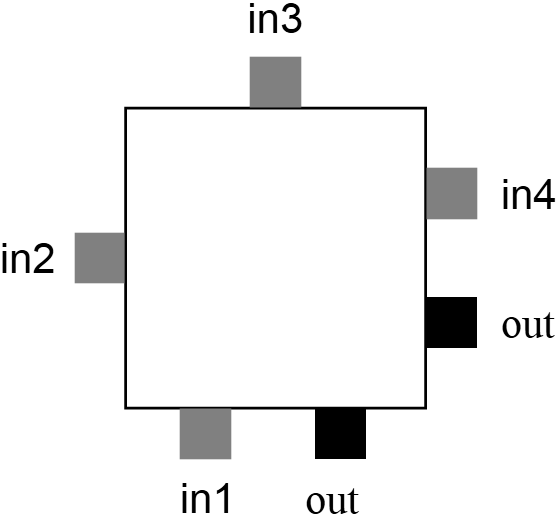
\includegraphics[scale=0.75]{FpgaLogicBlockPins.png}  
	\caption{Расположение контактов логического блока FPGA}
	\label{fig:FpgaLogicBlockPins}
\end{figure}

Входы расположены на отдельных сторонах логического блока, выходной контакт может трассироваться в двух каналах: либо справа от блока, либо снизу. Выходные контакты каждого логического блока могут соединяться с трассировочными сегментами в смежных каналах. Аналогично, контактная площадка блока ввода-вывода (pad) может соединяться с трассировочным элементом в любом смежном канале. Например, верхняя контактная площадка чипа может соединяться с любым из W проводников (где W - ширина канала) в горизонтальном канале, расположенном непосредственно под ним~\cite{Wiki_FPGA}.

Как правило, трассировка ППВМ несегментирована, то есть каждый сегмент проводника соединяет только один логический блок с переключательным блоком. Из-за огибания программируемых переключателей в переключательном блоке трассировка получается более длинной. Для увеличения скорости внутрисистемных соединений, в некоторых архитектурах ППВМ используются более длинные трассировочные соединения между логическими блоками~\cite{Wiki_FPGA}.

\begin{figure}[ht]
	\centering
	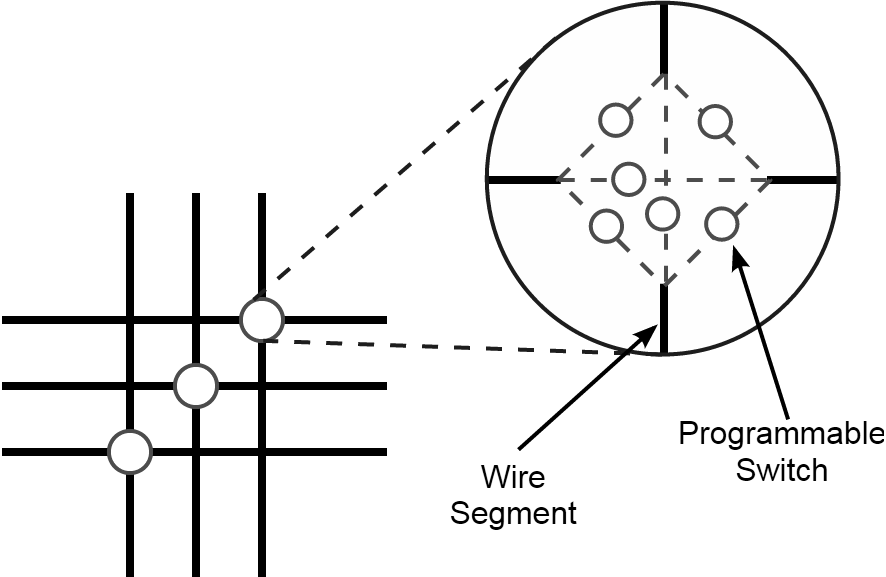
\includegraphics[scale=0.6]{FpgaSwitchBox.png}  
	\caption{Топология переключательного блока FPGA}
	\label{fig:FpgaSwitchBox}
\end{figure}

В месте пересечения вертикальных и горизонтальных каналов создаются переключательные блоки. При такой архитектуре для каждого проводника, входящего в переключательный блок, существуют три программируемых переключателя, которые позволяют ему подключаться к трём другим проводникам в смежных сегментах канала. Модель или топология выключателей, используемая в этой архитектуре, является планарной или доменной топологией переключательных блоков. В этой топологии проводник трассы номер один подключается только к проводнику трассы номер один в смежных каналах, проводник трассы номер 2 подключается только к проводникам трассы номер 2 и так далее. На рисунке~\ref{fig:FpgaSwitchBox} показаны соединения в переключательном блоке~\cite{Wiki_FPGA}.

% **************************************************
\subsection{Отладочная плата \boardname{}}
\boardname{}~--- это отладочная плата которая подходит как для обучения обучения, так и для разработки и тестирования систем на базе FPGA. Главный элемент данной платы~--- это FPGA-чип EP4CE115, который имеет более 100 тысяч логических элементов и является топовым внутри серии Cyclone~IV. Данный чип имеет следующие характеристики:
\begin{itemize}
	\item 114 480 логических элементов;
	\item 3 888 Кбит встроенной памяти;
	\item 266 встроенных умножителей разрядностью 18 x 18 бит;
	\item 4 блока ФАПЧ общего назначения.
	\item 528 пользовательских цифровых входов/выходов.
\end{itemize}

Отличительными особенностями платы являются:
\begin{itemize}
	\item 50 МГц тактовый генератор, 2 разъёма SMA для входа/выхода тактовой частоты;
	\item 2 МБайт SRAM, 2x64 МБайт SDRAM, 8 МБайт Flash, разъём для SD карт;
	\item 4 кнопки, 18 микропереключателей;
	\item 18 красных и 9 зелёных пользовательских светодиодов, ЖКИ 16x2;
	\item 24-разрядный аудио-кодек CD-качества с разъёмами линейного входа/выхода и микрофонного входа;
	\item VGA ЦАП (8-разрядный высокопроизводительный трёхканальный) с выходным VGA разъёмом;
	\item TV декодер (NTSC/PAL/SECAM) и разъём TV входа;
	\item 2 Gigabit Ethernet PHY с разъёмом RJ45;
	\item USB Host/ Slave контроллер с разъёмами USB type A и type B;
	\item Приёмопередатчик RS-232 с 9-контактным разъёмом, разъём PS/2 мыши/клавиатуры, ИК приёмник для пульта ДУ;
	\item 40-контактный разъём расширения с диодной защитой. Разъём для подключения мезонинных модулей (HSMC).
\end{itemize}

Особенно стоит отметить возмжность приобретение данной платы по студенческой цене, которая ниже, чем розничная стоимость отдельного FPGA-чипа, который установлен на плате.

В комплект платы \boardname{} входят следующие компоненты:
\begin{itemize}
	\item Плата DE2-115;
	\item USB кабель для программирования и управления FPGA;
	\item Системный CD, содержащий документацию на DE2-115 и материалы технической поддержки разработок;
	\item Комплект CD, содержащий ознакомительные версии ПО Altera’s Quartus II Web Edition и Nios II Embedded Design Suit;
	\item Пакет с 6 резиновыми (силиконовыми) колпачками для стоек платы DE2-115;
	\item Прозрачная пластмассовая защитная пластина для платы;
	\item 12 В сетевой источник питания;
	\item Пульт дистанционного управления.
\end{itemize}

Изображения платы с обеих сторон и расположение на ней компонентов показаны на рисунке~\ref{fig:FpgaBoard}.

\begin{figure}[ht]
\centering
  \begin{subfigure}[b]{1\textwidth} 
    \centering
    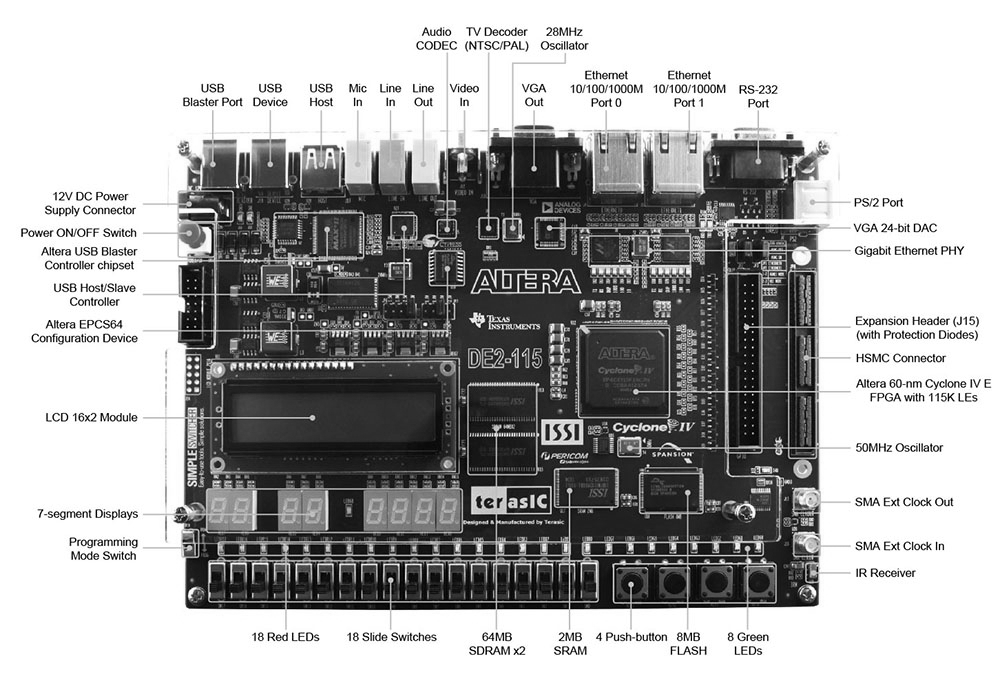
\includegraphics[scale=0.45]{FpgaBoardTop.jpg}  
    \caption{}
  \end{subfigure}
  \begin{subfigure}[b]{1\textwidth} 
    \centering
    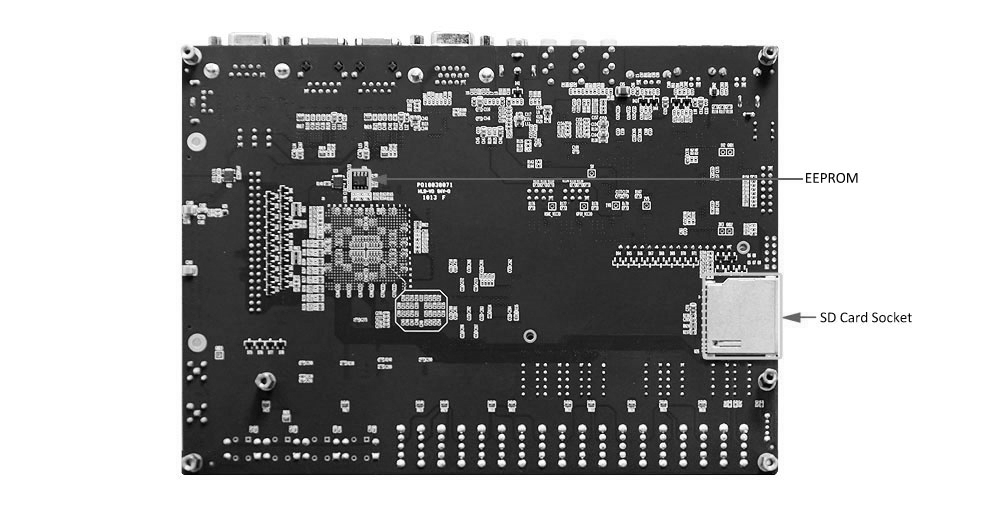
\includegraphics[scale=0.45]{FpgaBoardBottom.jpg}  
    \caption{}
  \end{subfigure}
  \caption{ Изображение платы \boardname{} и расположение на ней компонентов:
			а "--- с задней стороны;
			б "--- с передней стороны.}
  \label{fig:FpgaBoard}
\end{figure}
